\documentclass[preprint,12pt]{elsarticle}

%% Use the option review to obtain double line spacing
%\documentclass[authoryear,preprint,review,12pt]{elsarticle}

%% Use the options 1p,twocolumn; 3p; 3p,twocolumn; 5p; or 5p,twocolumn
%% for a journal layout:
%% \documentclass[final,1p,times]{elsarticle}
%% \documentclass[final,1p,times,twocolumn]{elsarticle}
%% \documentclass[final,3p,times]{elsarticle}
%% \documentclass[final,3p,times,twocolumn]{elsarticle}
%% \documentclass[final,5p,times]{elsarticle}
%% \documentclass[final,5p,times,twocolumn]{elsarticle}

%% For including figures, graphicx.sty has been loaded in
%% elsarticle.cls. If you prefer to use the old commands
%% please give \usepackage{epsfig}

%% The amssymb package provides various useful mathematical symbols
\usepackage{amssymb}
%% The amsthm package provides extended theorem environments
%%\usepackage{amsthm}
\usepackage{amsmath}

\usepackage{url}

\usepackage{algorithmicx}
\usepackage{algorithm}
\usepackage[noend]{algpseudocode}

\usepackage{subcaption}

%% The lineno packages adds line numbers. Start line numbering with
%% \begin{linenumbers}, end it with \end{linenumbers}. Or switch it on
%% for the whole article with \linenumbers.
%% \usepackage{lineno}

\journal{Pattern Recognition}

\begin{document}

\begin{frontmatter}

%% Title, authors and addresses

%% use the tnoteref command within \title for footnotes;
%% use the tnotetext command for theassociated footnote;
%% use the fnref command within \author or \address for footnotes;
%% use the fntext command for theassociated footnote;
%% use the corref command within \author for corresponding author footnotes;
%% use the cortext command for theassociated footnote;
%% use the ead command for the email address,
%% and the form \ead[url] for the home page:
%% \title{Title\tnoteref{label1}}
%% \tnotetext[label1]{}
%% \author{Name\corref{cor1}\fnref{label2}}
%% \ead{email address}
%% \ead[url]{home page}
%% \fntext[label2]{}
%% \cortext[cor1]{}
%% \address{Address\fnref{label3}}
%% \fntext[label3]{}

\title{The Weight-Shape Decomposition of Density Estimates: A Framework for Clustering and Image Analysis Algorithms}

%% use optional labels to link authors explicitly to addresses:
%% \author[label1,label2]{}
%% \address[label1]{}
%% \address[label2]{}

\author[tau]{Lior Deutsch}
\ead{sliorde@gmail.com}
\author[tau]{David Horn\corref{cor}}
\ead{horn@tau.ac.il}
\cortext[cor1]{Corresponding author}

\address[tau]{Tel Aviv University, Tel Aviv, Israel}

\begin{abstract}
We propose an analysis scheme which addresses the Parzen-window and mixture model methods for estimating the probability density function of data points in feature space. Both methods construct the estimate as a sum of kernel functions (usually Gaussians). By adding an entropy-like function we prove that the probability distribution is a product of a weight function and a shape distribution. This Weight-Shape decomposition leads to new interpretations of established clustering algorithms. Furthermore, it suggests the construction of three different clustering schemes, which are based on gradient-ascent flow of replica points in feature space. Two of these are quantum clustering (QC) and the mean-shift (MS) algorithm. The third algorithm is based on maximal-entropy. In our terminology they become Maximal Shape Clustering (MSC), Maximal Probability Clustering (MPC) and Maximal Weight Clustering (MWC), correspondingly. We demonstrate the different methods and compare them to each other on one artificial example and two natural data sets. We also apply the Weight-Shape decomposition to image analysis. The shape distribution acts as an edge detector. It serves to generate contours, as demonstrated on face images. Furthermore, it allows for defining a convolutional Shape Filter.

\end{abstract}

\begin{keyword}
density estimate \sep quantum clustering \sep mean-shift clustering \sep maximum entropy \sep image contour extraction

%% PACS codes here, in the form: \PACS code \sep code

%% MSC codes here, in the form: \MSC code \sep code
%% or \MSC[2008] code \sep code (2000 is the default)
\end{keyword}

\end{frontmatter}

%% \linenumbers




\section{Introduction}
\label{introduction}
The Parzen-window approach \cite{parzen1962estimation} is a method attributing to each data point in feature space a kernel. The sum of all kernels is perceived as an estimate of the probability density function (pdf) of the data. The most popular choice of kernels is a Gaussian with a common width. This approach has been employed in various clustering studies: Roberts \cite{roberts1997} proposed to view the peaks of the resulting probability density as possible locations of cluster centers, thus establishing a heuristic clustering method. He proposed using stability of these clusters under variation of the kernel width as a criterion for useful clustering schemes. Searching for peaks of the Parzen-window density function has also been proposed within the mean-shift algorithm in \cite{cheng1995} and in \cite{comaniciu2002}. Quantum Clustering (QC) \cite{horn2001} has employed this Parzen-window and transformed it into a potential function whose minima describe clustering centers. Although the history of the Parzen window approach dates back to 1962, it remains a useful tool of machine learning, as indicated in a recent survey of clustering algorithms \cite{xu2015comprehensive}. An older review puts it in context of many other methods in statistical pattern recognition \cite{jain2000statistical}.

Mixture-models \cite{titterington1985} are parametric methods for pdf estimation. Although not usually considered kernel methods, these models also position kernel functions in feature space. Their number is much smaller than the number of data points, and their locations and parameters are optimized, typically using the maximum likelihood criterion. 

Both types of models share the property that a pdf is estimated using a superposition of kernel functions, located at different points in feature space. We introduce a Weight-Shape decomposition of the pdf estimator, which is valid for all of them. This is achieved by a novel entropy function which is defined in addition to the Parzen probability function. The difference between the two defines yet a third function, which allows us to derive the Weight-Shape decomposition of the density function. The latter is the product of two factors: Weight, which has non-local information about the number of neighbors to a point, and Shape, which reflects local properties which are unbiased by Weight.

Kernels are also used in the realm of image processing. For example, the scale space approach \cite{witkin1984} filters the image with kernels of various scales. Appropriate kernels can be chosen to find various features of the image, such as edges or ridges. Analysis of the filtered images reveals these structures at various scales.

We employ the Weight-Shape decomposition for defining three families of clustering methods: one is based on probability maximization, and, as such, is analogous to the mean-shift algorithm. Another is based on Shape maximization, and turns out to coincide with QC for Gaussian kernels. The third is based on Weight maximization, which also implies entropy maximization. All are developed within a common framework of gradient ascent of replica points moving within feature space.

We also employ the Weight-Shape decomposition for image analysis. We will demonstrate that the shape distribution can be used to extract contour representation of an image, e.g. line caricatures of faces. Numerical analysis is carried out by employing a convolutional Shape Filter.













\section{The Weight-Shape Decomposition}
\label{wsd}
Let us consider the expression
\begin{equation}\label{sum_of_kernels}
  \Psi\left(\mathbf{x}\right) = \sum_i K_i \left( \mathbf{x}-\boldsymbol{\mu}_i \right) 
\end{equation}
which is a sum over kernels, where $\mathbf{x},\boldsymbol{\mu}_i\in\mathbb{R}^d$. We refer to $\mathbb{R}^d$ as \textit{feature space}. The \textit{kernels} $K_i$ are functions $\mathbb{R}^d\rightarrow\mathbb{R}$, and $\boldsymbol{\mu}_i$ are \textit{kernel centers}. The latter may be data points but, in general, can be different. For example, in the case of a Gaussian mixture model, $\Psi(\mathbf{x})$ represents a pdf, and the kernels are the Gaussians
\begin{equation}\label{gaussian_kernel}
  K_i \left( \mathbf{x}-\boldsymbol{\mu}_i \right) = \pi_i\exp\left(-\frac{1}{2}\left(\mathbf{x}-\boldsymbol{\mu}_i\right)^T\boldsymbol{\Sigma}_i^{-1}\left(\mathbf{x}-\boldsymbol{\mu}_i\right)\right),
\end{equation}
The model parameters of the pdf are the Gaussian center locations $\boldsymbol{\mu}_i$, the covariance matrices $\boldsymbol{\Sigma}_i$ and the mixing proportions $\pi_i$. Typically, the maximum likelihood criterion is used to assign values to the model parameters. In the case of a Parzen pdf estimator, all kernels $K_i$ are usually taken equal, and $\boldsymbol{\mu}_i=\mathbf{x}_i$ are the data points. $\Psi\left(\mathbf{x}\right)$ serves then as a non-parametric estimation of the pdf, depending on a common width $\sigma$.

We define a probability space that associates any point ${\mathbf{x}}$ in feature space with all kernel centers:
\begin{equation}\label{probability}
  p_i\left(\mathbf{x}\right)=\frac{K_i\left(\mathbf{x}-\boldsymbol{\mu}_i\right)}{\Psi\left(\mathbf{x}\right)}.
\end{equation}
Obeying $\sum_ip_i\left(\mathbf{x}\right)=1$. In the case of a Gaussian mixture model, these probabilities are the posterior probabilities, following from Bayes rule. We define an \textit{entropy function} of the probability space at point $\mathbf{x}$
\begin{equation}\label{entropy}
  H\left(\mathbf{x}\right)=-\sum_i p_i\left(\mathbf{x}\right)\log p_i\left(\mathbf{x}\right)
\end{equation}
and an \textit{average energy} function as 
\begin{equation}\label{average_energy}
  V\left(\mathbf{x}\right)= H\left(\mathbf{x}\right) - \log\Psi\left(\mathbf{x}\right) = -\sum_i p_i\left(\mathbf{x}\right)\log K_i \left( \mathbf{x}-\boldsymbol{\mu}_i \right).
\end{equation}
For the Gaussian kernel $K_i\left(\mathbf{x}\right)=\exp\left(-\frac{\mathbf{x}^2}{2\sigma^2}\right)$, it reduces to
\begin{equation}\label{average_energy_gaussian}
  V\left(\mathbf{x}\right)= \sum_i \frac{\left(\mathbf{x}-\boldsymbol{\mu}_i\right)^2}{2\sigma^2} p_i\left(\mathbf{x}\right).
\end{equation}
$V\left(\mathbf{x}\right)$ is the average squared-distance at point $\mathbf{x}$. Eq. \ref{average_energy_gaussian} has an analogy in statistical mechanics \cite{jaynes1957} where $V$ is the average energy of a canonical ensemble, $H$ is the entropy and $\Psi$ is the partition function. Note however that while in statistical mechanics these three functions are global characteristics of a system, here they are defined as fields, i.e. functions of $\mathbf{x}$, any point in feature space.

Introducing the functions $W\left(\mathbf{x}\right)=\exp\left(H\left(\mathbf{x}\right)\right)$ and $S\left(\mathbf{x}\right)=\exp\left(-V\left(\mathbf{x}\right)\right)$, we may rewrite Eq. \ref{average_energy} as
\begin{equation}\label{weight_shape_decomposition}
  \Psi\left(\mathbf{x}\right)=W\left(\mathbf{x}\right)S\left(\mathbf{x}\right)
\end{equation}
to which we refer as the \textit{Weight-Shape decomposition} of the pdf. $S\left(\mathbf{x}\right)$ represents the shape of $\Psi\left(\mathbf{x}\right)$, and the perplexity $W\left(\mathbf{x}\right)$represents the weight. Their properties are demonstrated in Fig. \ref{1d_example}, which depicts the functions for synthetic data set. In the upper panel there are $300$ randomly generated points with a $1:2$ bias between left and right. The lower panel displays the changes caused by additional $25$ points generated by a Gaussian of width $0.2$ around the origin. The Parzen function is constructed using Gaussian kernels with width $\sigma=1$,$1.5$ and $2$, and it is presented together with its $W\left(\mathbf{x}\right)$ and $S\left(\mathbf{x}\right)$ components. The graphs in the upper panel show that the $1:2$ bias does not affect $S\left(\mathbf{x}\right)$. On the other hand, $W\left(\mathbf{x}\right)$ displays more correctly than $\Psi$ the $1:2$ weights of the data. $S\left(\mathbf{x}\right)$ describes the shape of the two sources for the higher values of $\sigma$, when the other two functions fail to do it. The lower panel demonstrates that only $S$ is sensitive enough to notice the additional data around the origin.

\begin{figure}[t]
\centering
\begin{subfigure}{.32\linewidth}{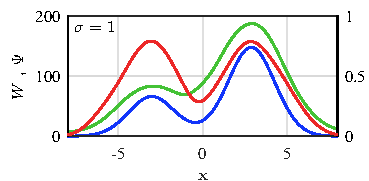
\includegraphics[width=1\linewidth]{fig1a.pdf}}\end{subfigure}
\begin{subfigure}{.32\linewidth}{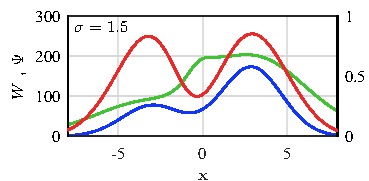
\includegraphics[width=1\linewidth]{fig1b.pdf}}\end{subfigure}
\begin{subfigure}{.32\linewidth}{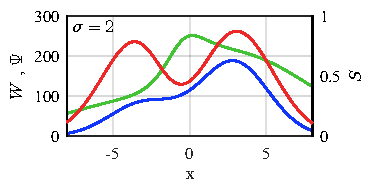
\includegraphics[width=1\linewidth]{fig1c.pdf}}\end{subfigure}
\begin{subfigure}{.32\linewidth}{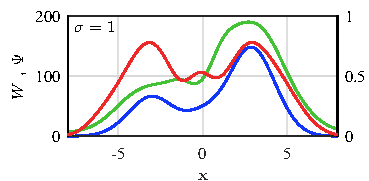
\includegraphics[width=1\linewidth]{fig1d.pdf}}\end{subfigure}
\begin{subfigure}{.32\linewidth}{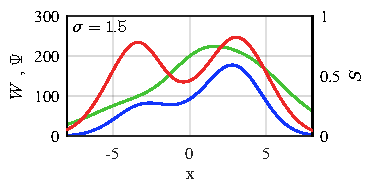
\includegraphics[width=1\linewidth]{fig1e.pdf}}\end{subfigure}
\begin{subfigure}{.32\linewidth}{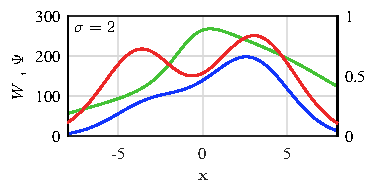
\includegraphics[width=1\linewidth]{fig1f.pdf}}\end{subfigure}
\begin{subfigure}{0.32\linewidth}{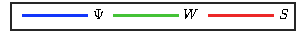
\includegraphics[width=1\linewidth]{legend.pdf}}\end{subfigure}
\caption{The Parzen estimator $\Psi$, with its Weight $W$ and Shape $S$ components, for a synthetic $1$-dimensional data set, displayed for three different values of $\sigma$. Upper panel: randomly generated points with Gaussians of width $1$, $100$ points around $\mathbf{x}=-3$ and $200$ points around $\mathbf{x}=3$. Lower panel: adding to the above $25$ points around $\mathbf{x}=0$, randomly generated by Gaussian of width $0.2$. The left axes denote values of $\Psi$ and $W$, and the right axes denote values of $S$.}
\label{1d_example}
\end{figure}

















\subsection{Weight-Shape Decomposition in Fuzzy Clustering}
\label{fuzzy}
Our first application will be to fuzzy $c$-means \cite{bezdek1984}. The objective is to minimize the total energy
\begin{equation}\label{Vtot}
  V_\textrm{tot} = \sum_{i=1}^n\sum_{j=1}^k \left( \mathbf{x}_i-\boldsymbol{\mu}_j \right)^2 p_{ij},
\end{equation}
where $\mathbf{x}_i$ are data points and $\boldsymbol{\mu}_j$ are cluster centers. $p_{ij}$ are probabilities obeying $\sum_{j=1}^{k}p_{ij}=1$, which designate fuzzy cluster memberships. The proposed algorithm in \cite{li1995,rose1990} is carried out in two repetitive steps:\\
\textbf{1)} For a given set of $\boldsymbol{\mu_j}$, update all $p_{ij}$ so as to maximize the total entropy
\begin{equation}\label{Htot}
  H_\textrm{tot} = -\sum_{i=1}^n\sum_{j=1}^k p_{ij} \log p_{ij},
\end{equation}
while keeping $V_\textrm{tot}$ fixed. This gives a least-biased probability distribution.\\
\textbf{2)} For a given set of $p_{ij}$, update all $\boldsymbol{\mu_j}$ by minimizing $V_\textrm{tot}$.\\
Using Eq. \ref{probability} one may represent the optimal solutions as $p_{ij}=p_j\left(\mathbf{x}_i\right)$ with a Gaussian kernel. This leads to
\begin{equation}\label{Htot_minus_Vtot}
  H_\textrm{tot}-V_\textrm{tot} = \sum_i H\left(\mathbf{x}_i\right)-\sum_i V\left(\mathbf{x}_i\right)=\sum_i \log\Psi\left(\mathbf{x}_i\right),
\end{equation}
where $\Psi\left(\mathbf{x}_i\right)=\sum_{j=1}^k \exp\left(-\frac{\left(\mathbf{x}-\boldsymbol{\mu}_j\right)^2}{2\sigma^2}\right)$. Treating $\Psi\left(\mathbf{x}_i\right)$ as a pdf estimation, $\sum_i \log\Psi\left(\mathbf{x}_i\right)$ is the log-likelihood of the data, and steps \textbf{1} and \textbf{2} each increase a different component of it. Thus, this algorithm is an expectation-maximization algorithm for maximizing the likelihood of a Gaussian mixture model.






















\subsection{Weight-Shape Decomposition in Quantum Clustering}
\label{qc}
In quantum clustering (QC) \cite{horn2001}, one uses the Parzen pdf with Gaussian kernels centered at all data-points ($\boldsymbol{\mu}_i=\mathbf{x}_i$). The pdf is assumed to obey the Schr{\"o}dinger equation
\begin{equation}\label{Schrodingers_equation}
  \left(-\frac{\sigma^2}{2}\boldsymbol{\nabla}^2+V\left(\mathbf{x}\right)-\frac{d}{2}\right)\Psi\left(\mathbf{x}\right)=0,
\end{equation}
thus defining $V\left(\mathbf{x}\right)$ to be a transform of $\Psi\left(\mathbf{x}\right)$:
\begin{equation}\label{Schrodingers_equation_potential}
  V\left(\mathbf{x}\right)=\frac{\sigma^2}{2}\frac{\left(\boldsymbol{\nabla}^2\Psi\right)\left(\mathbf{x}\right)}{\Psi\left(\mathbf{x}\right)}+\frac{d}{2}
\end{equation}
$d$ is the dimension of feature space. The same equation can be derived from Eqs. (\ref{sum_of_kernels}) and (\ref{average_energy_gaussian}) for the Gaussian kernel. Thus the quantum potential is identical to the average energy function $V\left(\mathbf{x}\right)=-\log S\left(\mathbf{x}\right)$. In the QC algorithm, replicas of the data points start off at the loci of all data points, and are made to obey gradient descent flow to arrive at local minima of $V\left(\mathbf{x}\right)$. Hence we conclude that QC serves to locally-maximize the shape function. Replica points that end up in the same extremum are grouped as a cluster. In \cite{horn2001} it was argued that local minima of $V\left(\mathbf{x}\right)$ provide successful alternatives to local maxima of $\Psi\left(\mathbf{x}\right)$, which is the objective of mean-shift clustering. We can argue now that $V\left(\mathbf{x}\right)$ has the advantage of filtering out the weight information from $\Psi\left(\mathbf{x}\right)$, thus allowing for an unbiased analysis.




























\section{Replica Flow Dynamics and Clustering Algorithms}
\label{replica}
Adopting replica flow dynamics as a clustering methodology we realize that it can serve as a common underlying principle defining three families of algorithms, maximizing probability, Weight or Shape. Maximal Probability Clustering (MPC) has the same objective function as the mean-shift algorithm \cite{cheng1995}. Maximal Shape Clustering (MSC) coincides, in the case of Gaussian kernels, with QC. Maximal Weight Clustering (MWC) is a novel method which follows naturally from our formalism. We refer to the three algorithms generically as MXC, where X= P, W or S. All three methods are carried out through repeated application of a gradient ascent updating step to replica points

\begin{equation}\label{gradient_descent_step}
  \mathbf{x}_i' \gets \mathbf{x}_i'+\eta\left(\boldsymbol{\nabla}\chi\right)\left(\mathbf{x}_i'\right),
\end{equation}

where $\chi$ stands for any one of the three fields $\chi \in \{\Psi,W,S\}$, defining the three clustering methods MXC, for X= P, W or S, respectively. $\eta$ is a small parameter to be chosen by the user. This formulation allows the use of Newton's method, quasi-Newton methods, line search, etc. The replica points start off at the positions of the data points and converge onto cluster centers. Their starting-off positions identify clusters of the original data points. See the pseudo-code of Algorithm \ref{MXC} for details.

\begin{algorithm}
\caption{MXC}\label{MXC}
\algblockdefx{MRepeat}{EndMRepeat}{\textbf{repeat }}{\textbf{end repeat}}
\algblockdefx{MFor}{EndMFor}{\textbf{for }}{\textbf{end for}}
\begin{algorithmic}[1]
\State define $\chi\in \{\Psi,W,S\}$ on the basis of the data points
\MFor each data point $\mathbf{x}_i$:
	\State $\mathbf{x}_i' \gets \mathbf{x}_i$
	\MRepeat until convergence:
		\State $\mathbf{x}_i' \gets \mathbf{x}_i'+\eta\left(\boldsymbol{\nabla}\chi\right)\left(\mathbf{x}_i'\right)$  
	\EndMRepeat
\EndMFor
\State group replica points that converged onto the same maximum and define them, as well as the original data which they stand for, as a single cluster
\end{algorithmic}
\end{algorithm}

We introduce also hierarchical versions of the three algorithms, HMXC. They start out with some small value of $\sigma$, and use the clusters which are being formed as sources of new replica points, replacing the older replica-points which were merged into the cluster (but remembering their identities) thus forming a one-to-many correspondence to the original data-points. The algorithm continues with MXC for higher $\sigma$, with new clusters and corresponding replica points being formed iteratively. The underlying fields  $\Psi$,$W$,$S$ continue to be evaluated through the original data points. See description in Algorithm \ref{HMXC}.

\begin{algorithm}
\caption{HMXC}\label{HMXC}
\algblockdefx{MRepeat}{EndMRepeat}{\textbf{repeat }}{\textbf{end repeat}}
\algblockdefx{MFor}{EndMFor}{\textbf{for }}{\textbf{end for}}
\begin{algorithmic}[1]
\State initialize a small value for $\sigma$
\State run MXC
\MRepeat until $\sigma$ is large enough:
	\State choose one representative replica point from each cluster, replacing all other replica points of the same cluster
	\State for each replica point, perform the gradient ascent step of MXC, (as in step of 4 MXC).
	\State group replica points into clusters as in step 8 of MXC.
	\State increase $\sigma$ by small amount.
\EndMRepeat
\end{algorithmic}
\end{algorithm}

A third possible version of all three algorithms is a blurred one - BMXC - where the underlying fields $\chi \in \{\Psi,W,S\}$ are re-evaluated, after each update of all replica points, on the new replica points instead of the original data-points. This is described in Algorithm 3. The concept of blurred versions of such algorithms has been introduced by Cheng \cite{cheng1995} in the context of the mean-shift algorithm.

\begin{algorithm}
\caption{BMXC}\label{BMXC}
\algblockdefx{MRepeat}{EndMRepeat}{\textbf{repeat }}{\textbf{end repeat}}
\algblockdefx{MFor}{EndMFor}{\textbf{for }}{\textbf{end for}}
\begin{algorithmic}[1]
\MFor each data points $\mathbf{x}_i$:
	\State $\mathbf{x}_i' \gets \mathbf{x}_i$
\EndMFor
\MRepeat until convergence:
	\State redefine $\chi$ on the basis of the current replica points (instead of data points).
	\MFor each replica point $\mathbf{x}_i'$:
		\State $\mathbf{x}_i' \gets \mathbf{x}_i'+\eta\left(\boldsymbol{\nabla}\chi\right)\left(\mathbf{x}_i'\right)$
	\EndMFor
\EndMRepeat
\State group replica points that fall into the same maximum and define this as a cluster.
\end{algorithmic}
\end{algorithm}

Discussions of the different algorithms are presented below, emphasizing their advantages and drawbacks. 































\subsection{Convergence of Gradient Ascent in MWC}
\label{convergence}
MWC may suffer from convergence problems. For example, if a cluster has $k$ members, and it is well separated from other clusters, then all points of the cluster are contained in a subspace of feature-space, whose dimension is limited by k. In the case of the Gaussian kernel, changes of W along any direction perpendicular to this subspace will not be affected by any point in the cluster. Hence, convergence onto the cluster is difficult to achieve through MWC along any perpendicular direction.
This leads to two bad effects on replica convergence in
MWC: \textbf{(1)} When a replica point reaches the maximum of the cluster, it may continue to wonder around in directions perpendicular to it under the effect of other clusters, leading to a delayed convergence procedure. \textbf{(2)} Since the movement of replica points is not limited to the cluster subspace, different replicas of the same cluster may not end up in the same final position, but may be scattered on perpendicular directions.
These problems can be mitigated by setting appropriate stopping conditions for the dynamics. We found that in large dimensions, including the example of clustering asteroid spectra, to obtain sensible results with MWC we had to do a relatively large number of trial-and-error iterations, changing thresholds of the stopping condition on each iteration. In contrast, MSC is less sensitive to the stopping condition.




















\subsection{Hierarchical Clustering Algorithms}
\label{hierarchical}
A data set may have structures at different scales, and we cannot expect clustering with one particular σ to reveal all these structures. The obvious way to deal with this difficulty is by running the clustering algorithm multiple times for a range of $\sigma$ values, representing different scales, and aggregating the results. If data points have errors assigned to them, $\sigma$ should preferably be larger than these errors.
The main problem with this approach is the inefficiency of the process. A more efficient approach is a hierarchical algorithm, HMXC, described in Alg. \ref{HMXC}. HMXC performs MXC between successive increments of $\sigma$, and whenever replica points fall into a cluster they are constrained to move together by MXC replica dynamics at larger $\sigma$.

There are two advantages to using hierarchical algorithms. The first is computational: as $\sigma$ grows, there are less and less replicas that undergo the process of gradient ascent, hence clustering at higher scales demands less computational steps.
The second advantage is conceptual: clusters obtained from all values of $\sigma$ form a hierarchical tree; thus if at a small scale two data points are members of the same cluster, they stay in one cluster also for larger scales. Hierarchy is not guaranteed when performing ab initio clustering on different scales $\sigma$. Nonetheless we find that the hierarchical and non-hierarchical approaches lead to similar results.











\subsection{Blurring Flow Dynamics}
\label{blurring}
 A motivation for blurring is that after each replica point has been updated, it is a bit closer to its presumed cluster center, and therefore may serve as a better estimator of the actual pdf of the data. Disadvantages of the blurring process are the following:\\ 
\textbf{(1)} the dynamics does not necessarily converge.  \\
\textbf{(2)} It is no longer possible to assign novel data points to previously derived clusters since the fields $\chi$ are modified in a fashion which depends on replica dynamics. \\
\textbf{(3)} The dynamics and final positions of the replica depend on the precise prescription used for gradient ascent, thus adding more degrees of freedom to the algorithm.


























\section{Analytic Cluster Attractors}
\label{analytic}
Whereas conventionally one searches for replica convergence onto cluster centers, one may also account convergence onto strings in analysis of big data \cite{weinstein2013}. Here we demonstrate the mathematical formats of a point-attractor and a line-attractor, which allow us to develop an intuition for replica convergence. We use the following definition: given the attractor, look for the dynamics which play out when a replica point starts out close to the attractor. If some of our clustering procedures are such that the replica points converge onto the attractor, the latter justifies its name.
























\subsection{The point attractor}
\label{point}
Assume a situation of $n_a$ data points coinciding at $\mathbf{x}=\mathbf{a}$, thus forming the Parzen estimator $\Psi=n_a \exp \left( -\frac{\left( \mathbf{x}-\mathbf{a} \right)^2}{2\sigma^2} \right)$. This leads to the \textit{point attractor} 
\begin{equation}\label{point_attractor}
  H=\log n_a,\quad V=\frac{\left(\mathbf{x}-\mathbf{a}\right)^2}{2\sigma^2},\quad \log\Psi=-\frac{\left(\mathbf{x}-\mathbf{a}\right)^2}{2\sigma^2}+\log n_a
\end{equation}
which is a valid approximation of the end result of every blurred algorithm leading to point clusters. Moreover, fields defined by Eq. (\ref{point_attractor}) will cause any replica point to flow into $\mathbf{x}=\mathbf{a}$ by using either MSC  or MPC. Note however that using MWC may be problematic, since the entropy is constant in the neighborhood of the attractor.

























\subsection{The Line Attractor}
\label{line}
Another interesting possibility is that of a line attractor. As an example consider a line in the range $[0,L]$ and construct an integral of Gaussian pdfs, which may be expressed in terms of $\textrm{erf}$ functions:
\begin{equation}\label{line_attractor_psi}
\begin{aligned}
  \Psi(x)=&\int_{0}^{L}\exp\left( -\frac{\left( x-\xi \right)^2}{2\sigma^2} \right) \mathrm{d} \xi=\\
  =&\sqrt{\frac{\pi \sigma^2}{2}}\left[\mathrm{erf}\left(\frac{x}{\sqrt{2}\sigma}\right)-\mathrm{erf}\left(\frac{x-L}{\sqrt{2}\sigma}\right)\right]
 \end{aligned}
\end{equation}

The corresponding continuous probability distribution, entropy and average energy are:
\begin{equation}\label{line_attractor_prob}
\begin{aligned}
  p_{\xi}(x)=&\frac{\exp\left( -\frac{\left( x-\xi \right)^2}{2\sigma^2} \right)}{\Psi(x)}, \quad 0\leq \xi \leq L \\
  H(x)=&\int_{0}^{L}p_{\xi}(x)\log p_{\xi}(x) \mathrm{d} \xi =\\
  =&-\frac{(L-x)\exp(-\frac{(L-x)^2}{2\sigma^2})+x\exp(-\frac{x^2}{2\sigma^2})}{2\Psi(x)}\\
  &+\log\Psi(x)+\frac{1}{2}\\
  V(x)=&-\frac{(L-x)\exp(-\frac{(L-x)^2}{2\sigma^2})+x\exp(-\frac{x^2}{2\sigma^2})}{2\Psi(x)}+\frac{1}{2}
 \end{aligned}
\end{equation}

Fig. \ref{line_attractor_fig} displays the behavior of these three fields as function of $x$, for $L=1$ and $\sigma=0.05$. For $\sigma \ll  L$ they are almost constant. This line attractor can be embedded in higher dimensions, by multiplying all kernels by $\exp \left( -\frac{\mathbf{y}^2}{2\sigma^2} \right)$ for any direction $\mathbf{y}$ which is perpendicular to $x$. There may be a problem with replica dynamics based on entropy, because displacements along $\mathbf{y}$ will encounter constant domains of $H$, as in the case of the point attractor. Hence only MPC and MSC can ensure that any replica-point converges onto a line, and even then this is an approximation which fails around the end points of the line.

A line attractor can also be made to have an arbitrary one-dimensional string shape. Although this is an ideal mathematical construct, it can represent a string-like potential valley in an approximate intermediate or final stage of replica dynamics. Such structures have been discovered in Dynamic Quantum Clustering (DQC) \cite{weinstein2009} analyses of big data \cite{weinstein2013}. In fact, the DQC convergence process, which is a quantum-mechanical analog of QC replica flow, has led to intermediate convergence of replica points onto $2$-dimensional structures, which have later separated into $1$-dimensional as well as $0$-dimensional (point) clusters.





\begin{figure}[t]
\centering
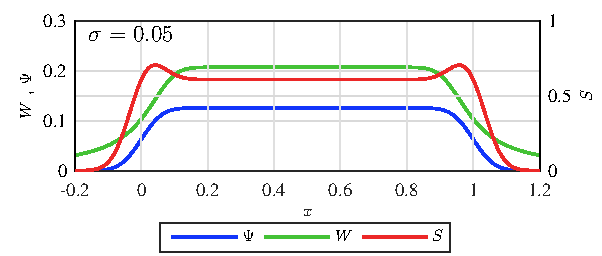
\includegraphics[width=0.6\linewidth]{fig2.pdf}
\caption{Display of the three fields along the line attractor.}
\label{line_attractor_fig}
\end{figure}


















\section{Clustering Studies of Natural Data Sets}
\label{natural}

























\subsection{The Crab Data Set}
\label{crabs}
Let us illustrate our method by applying the three different algorithms to the crab clustering problem which has been discussed in \cite{ben2001,horn2001}. This problem emerges from crab data included in Ripley's text book \cite{ripley1996}. The data consist of $200$ instances belonging to four equally-sized classes and defined in five-dimensional parameter space. Performing principal component analysis (PCA) \cite{jolliffe1986} on the data, and using a two-dimensional space defined by $\textrm{PC2}$ and $\textrm{PC3}$, the data exhibit observable differences between the classes, yet with large enough overlaps between them which render their clustering a challenging problem. We use this two-dimensional space as the feature space of our data set.

We have run the three different algorithms on this data set using a non-hierarchical approach. The clustering results can be compared with expert classifications \cite{ripley1996} employing the binary Jaccard score $J=\frac{n_{11}}{n_{11}+n_{10}+n_{01}}$, where $n_{11}$ stands for the number of pairs of points which reside together in one class in both classification schemes (i.e. expert classification and data clustering), and $n_{10}+n_{01}$ are numbers of pairs which belong to the same class in one of the two schemes but not in the other. The one parameter employed for all methods is $\sigma$, the width of the Gaussian kernels. For very large widths, the expected asymptotic value is $J=98/398$ , befitting one cluster and four classes. Fig. \ref{crabs}a displays the Jaccard scores of the different algorithms as function of $\sigma$. The best Jaccard scores are obtained for MSC, requiring relatively large $\sigma$ values.

Another advantage of MSC is its relative stability with respect to changes in $\sigma$. MWC and MPC reach their best $\sigma$ values, i.e. the ones leading to best Jaccard scores, much earlier. A different issue is the number of clusters that are obtained for the different algorithms, as function of the scale parameter $\sigma$. This is displayed in Fig.\ref{crabs}b. Note that the best MSC result (as determined by the Jaccard score) has six clusters, but there exists a large range of $\sigma$ which leads to a four-cluster solution, with very similar Jaccard scores. In fact, MSC is the only algorithm which provides the stable answer $4$ for a wide range of $\sigma$. Further analysis of this problem, and comparison of the different algorithms, is presented in \ref{crab_apndx}.




\begin{figure}[t]
\centering
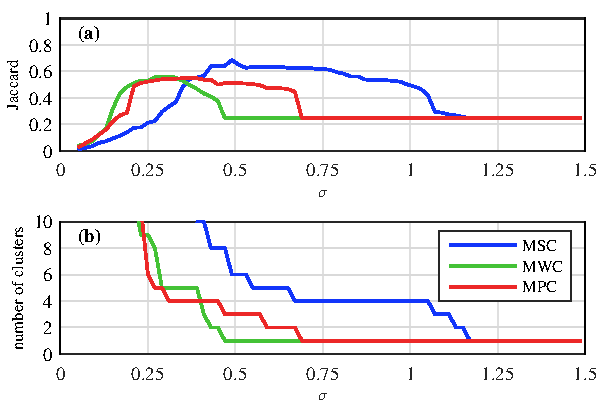
\includegraphics[width=0.6\linewidth]{fig3.pdf}
\caption{ \textbf{(a)} The Jaccard score, comparing our clustering results with expert classification. The clustering was using the three methods, on a range of $\sigma$ values. \textbf{(b)} The number of clusters, for each method and value of $\sigma$.}
\label{crabs}
\end{figure}





















\subsection{Analyses of Asteroid Spectra}
\label{asteroid}
Here we apply hierarchical clustering to another natural data set, composed of $1130$ observed spectra, measuring the reflection of sunlight in the near infra-red region, from $958$ main-belt and near-earth orbit asteroids. The data were obtained from \url{http://smass.mit.edu/} (accessed May 23, 2016) \cite{binzel2001,binzel2004,rivkin2004,rayner2003}. The spectra were interpolated to fit a grid of $76$ points between wave-lengths of $0.92\mu \textrm{m}$ to $2.42\mu \textrm{m}$ with step-size of $0.02\mu \textrm{m}$. The task at hand is clustering the $1130$ spectra, measured at $76$ wave-lengths. In other words, the data may be viewed as $1130$ vectors in a $76$ dimensional space.

We have applied HMWC and HMSC to this problem. In the absence of an oracle providing target classification, we choose a final value for $\sigma$ by visual inspection of the resulting clusters. The five largest clusters of HMWC are displayed in Fig. \ref{IR_HMWC} using $\sigma=0.14$. The total number of clusters, for this value of $\sigma$, is $111$. In addition, 316 spectra remained singletons. Fig. \ref{IR_HMSC} shows clustering results of HMSC, using $\sigma=0.15$. The resulting clusters have comparable sizes to those displayed for HMWC, but they do not coincide.

\begin{figure}[tb]
\centering
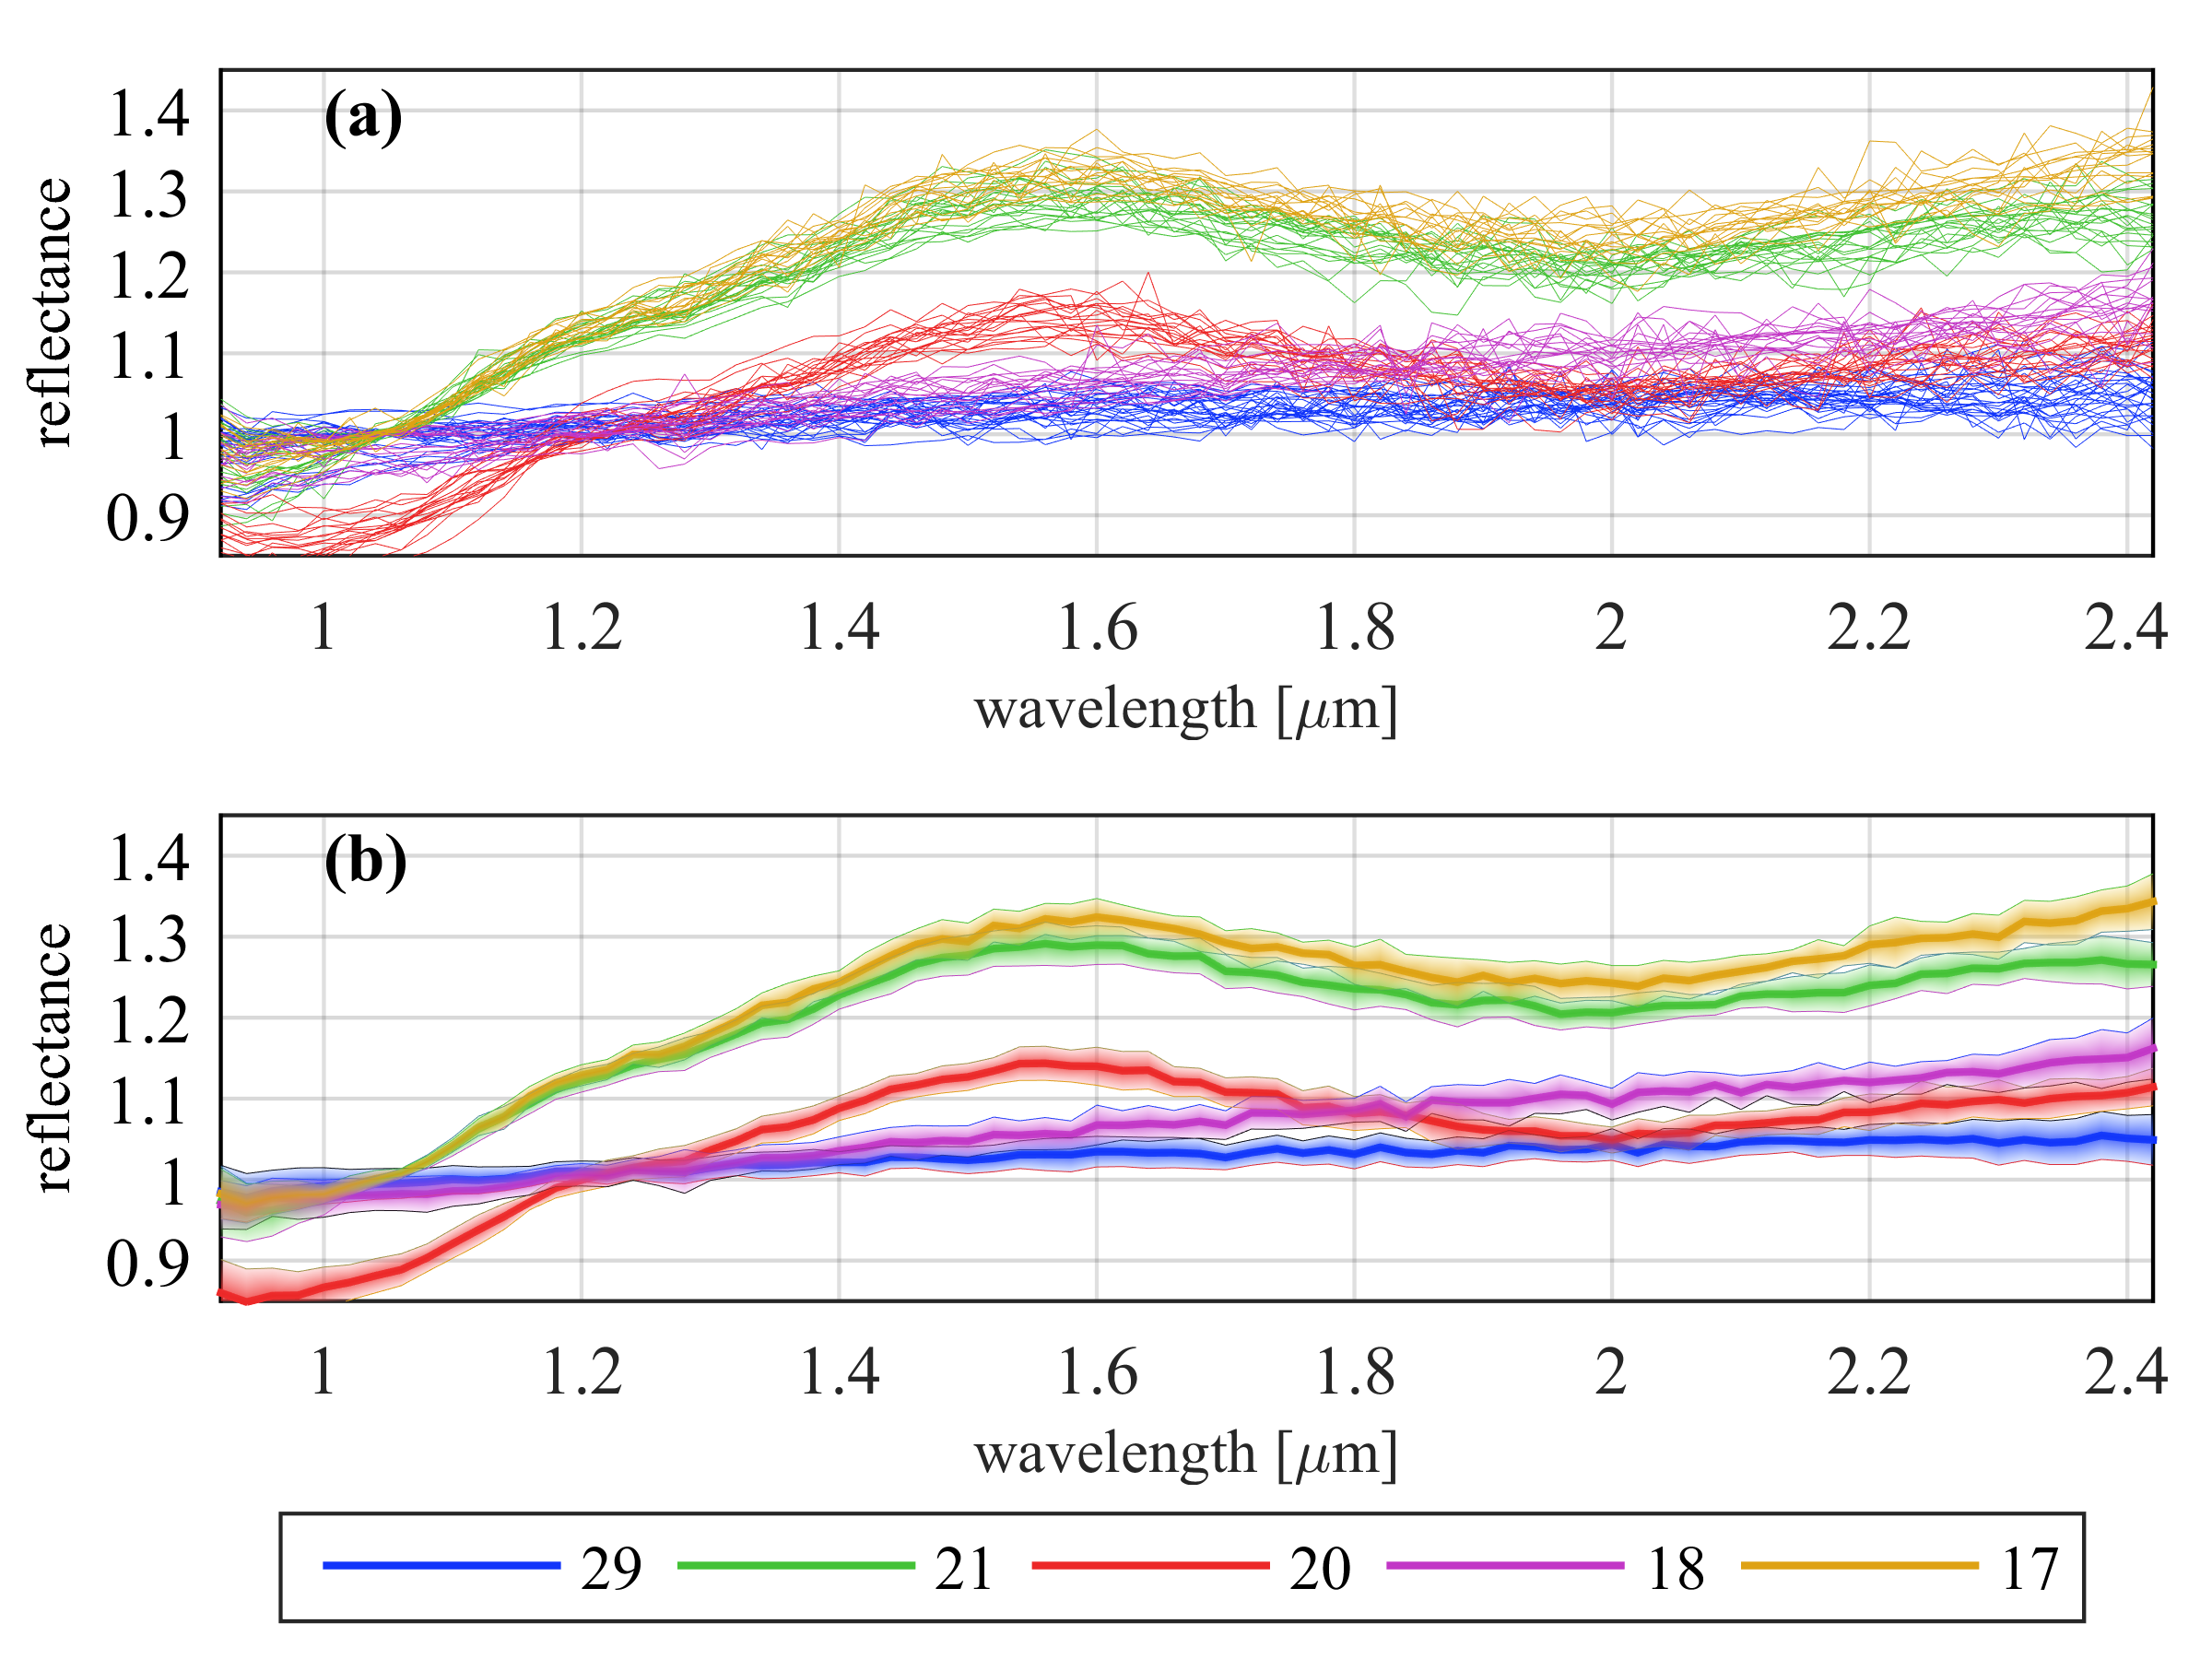
\includegraphics[width=0.6\linewidth]{fig4.png}
\caption{ The five largest clusters of asteroid IR spectra, obtained using HMWC. The initial value of $\sigma$ was $0.05$ and it was raised by $0.01$ on each iteration of the hierarchical algorithm. These results correspond to $\sigma=0.14$. The legend shows cluster sizes. \textbf{(a)}  The members of each cluster. \textbf{(b)} The average spectrum with $\pm\textrm{standard deviation}$ boundaries for each wavelength.}
\label{IR_HMWC}
\end{figure}

\begin{figure}[tb]
\centering
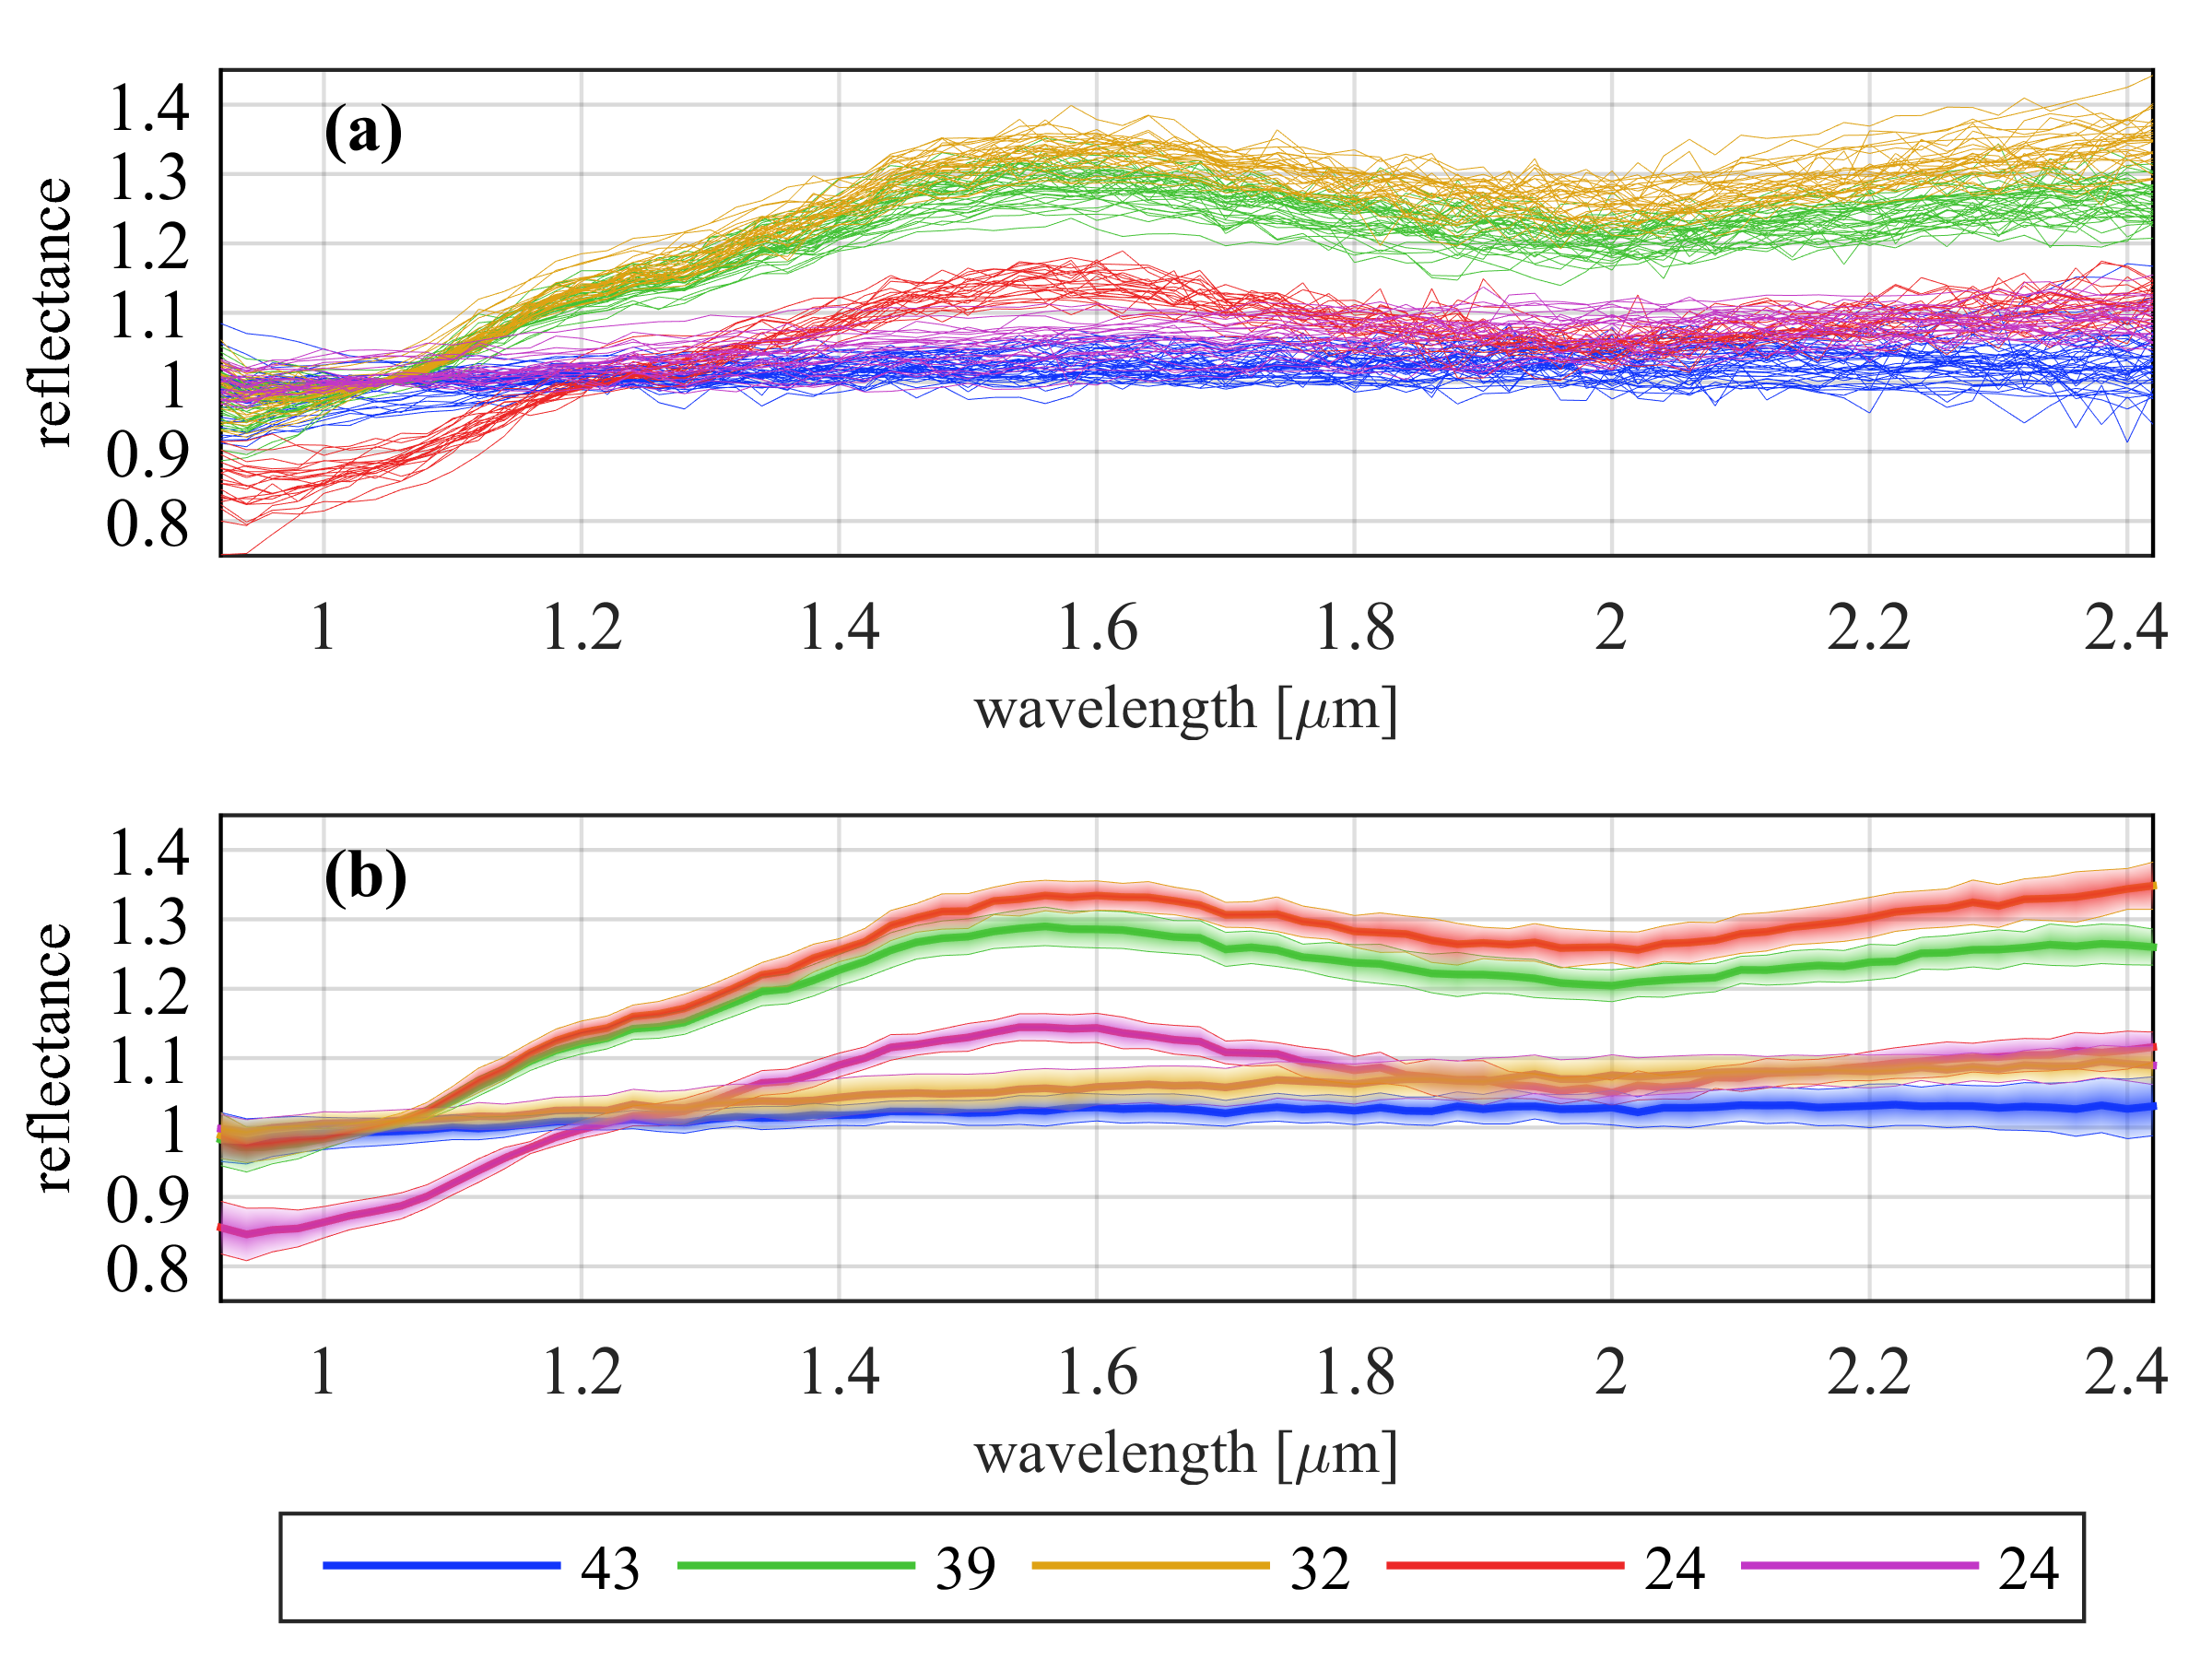
\includegraphics[width=0.6\linewidth]{fig5.png}
\caption{ The five largest clusters of asteroid IR spectra, obtained using HMSC. The initial value of $\sigma$ was $0.05$ and it was raised by $0.01$ on each iteration of the hierarchical algorithm. The results correspond to $\sigma=0.15$. The legend shows the cluster sizes. \textbf{(a)}  The members of each cluster. \textbf{(b)} The average spectrum with $\pm\textrm{standard deviation}$ boundaries for each wavelength.}
\label{IR_HMSC}
\end{figure}


The highest Jaccard score between HMWC and HMSC clusters in this problem turns out to be $J=0.3$. This is obtained for $\sigma=0.12$ in both methods, and the results are very similar to the ones displayed in Figs. \ref{IR_HMWC} and \ref{IR_HMSC}. In the absence of independent criteria (ground truth) it is difficult to claim that one method is better than the other. Nonetheless we note that larger clusters are obtained HMSC, which is an important advantage in classification exercises.

Similar data, consisting of asteroid spectra in the visible and near IR ranges, have been studied in \cite{deutsch2017quantum}. The results can be favorably compared to the Bus-DeMeo taxonomy \cite{demeo2009extension}, which was the latest attempt to form such clusters, in that the QC based scheme displays small variance in the wavy shapes between the different members in each cluster. This visual criterion is obviously satisfied by both figures \ref{IR_HMWC} and \ref{IR_HMSC}.
























\section{Weight-Shape Decomposition and Image Analysis}
\label{image}
The Parzen approach has been a major corner-stone for theory and practice of image analysis \cite{lindeberg1994}. It seems therefore natural to search for the novelties that the Weight-Shape decomposition has to offer.

Given a grayscale image intensity $0< I[m, n] <1$, with discrete indices $m$ and $n$ denoting pixel locations,  we define the (un-normalized) probability distribution as a convolution of the image $I$ with a kernel function $K$

\begin{equation}\label{psi_image}
  \Psi[m,n]=\sum_{k,l}K[m-k,n-l]I[k,l]=\left(I\ast K\right)[m,n],
\end{equation}

where $I\ast K$ symbolizes the convolution of $I$ and $K$. Correspondingly, we define $p_{k,l}[m,n]$ as the probability to assign pixel $[m,n]$ with each unit of the image in the pixel $[k,l]$:

\begin{equation}\label{prob_image}
  p_{k,l}[m,n]=\frac{K[m-k,n-l]}{\Psi[m,n]}.
\end{equation}

These probabilities obey $\sum_{k,l}p_{k,l}[m,n]I[k,l]=1$. The entropy and average energy may then be defined as
\begin{equation}\label{H_V_image}
\begin{aligned}
  H[m,n]=&-\sum_{k,l}I[k,l]p_{k,l}[m,n]\log p_{k,l}[m,n]\\
  V[m,n]=&H[m,n]-\log \Psi[m,n]=\frac{\left(I\ast L\right)[m,n]}{\left(I\ast K\right)[m,n]},
\end{aligned}
\end{equation}
where $L=-K\log K$. The Weight and Shape are defined by $W\left(\mathbf{x}\right)=\exp\left(H\left(\mathbf{x}\right)\right)$ and $S\left(\mathbf{x}\right)=\exp\left(-V\left(\mathbf{x}\right)\right)$ as before. $S$ may be viewed as a Shape Filter, defined in terms of the filters $K$ and $L$.
























\subsection{Using Shape for Contour Drawing}
\label{contour}
In our discussion of clustering methodologies we have put the emphasis on searching for maxima of the density function or its Weight component or its Shape distribution. Applying the same approach to image analysis we propose to emphasize the large components of the shape distribution, which will result in contour drawings, resembling line caricatures of images.
We demonstrate this approach on portraits of political leaders, shown in Fig. \ref{Trump} and Fig. \ref{leaders}. The grayscale pixel values were rescaled, after which a cutoff has been imposed on the strength of the shape signal. The probability drawing is the result of the density estimate, and the Weight component is very similar to it. Both are not very different from the original image for a low value of $\sigma$. The Shape of the image eliminates differences in brightness and enhances edges. Imposing a large cut-off on this spectrum of gray levels, one is lead to results exemplified in Fig. \ref{leaders}. Clearly the resulting shapes befit a line caricature of the original image.

The fact that $V$ in Eq. \ref{H_V_image}, has a non-linear form, which can be thresholded to achieve important features of the image, raises the possibility of using Shape (or $V$ itself) as a novel element to be incorporated in convolutional neural networks.

\begin{figure}[tbh]
\centering
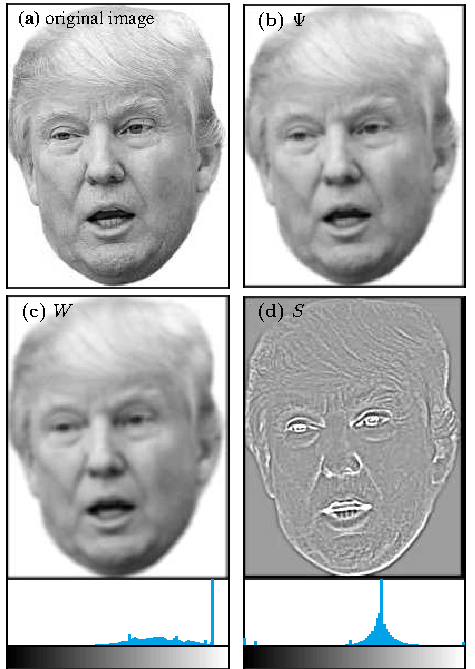
\includegraphics[width=.6\linewidth]{fig6.pdf}
\caption{\textbf{(a)} the original, grayscale image. Its size is $254\times198$. \textbf{(b)} The Parzen distribution, using a Gaussian filter with $\sigma=1.1$, truncated beyond a circular support of radius $10$. Before applying the filter, the image was rescaled to the range $[0.1,0.9]$. \textbf{(c)} The weight function, with a histogram of its grayscale values. \textbf{(d)} The shape distribution, with a histogram of its grayscale values. For display purposes, the shape image pixel values were truncated at the image's $1\%$ and $99\%$ percentiles, and the image is displayed inversely (high values are dark, low values are bright).}
\label{Trump}
\end{figure}

\begin{figure}[tbh]
\centering
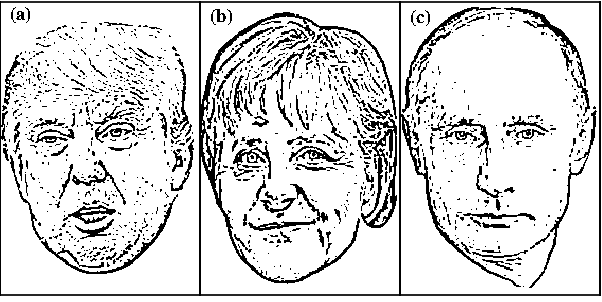
\includegraphics[width=0.6\linewidth]{fig7.pdf}
\caption{The results of imposing a cutoff on the shape image. The  processing employed in Fig. \ref{Trump}, was applied to each image using the same value of $\sigma$. All images were cut off at a shape value of $0.36$. \textbf{(a)} Image size: $254\times198$. \textbf{(b)} Image size: $267\times189$. \textbf{(c)} Image size: $268\times188$.}
\label{leaders}
\end{figure}



















\subsection{Evaluation of the Shape Filter}
\label{filter}
The forms of the filters $K$ and $L$, which appear in Eq. \ref{H_V_image}, are displayed in Fig. \ref{filters}. For practical reasons of computation, $K$ should be chosen to have a finite, small support. This raises a problem: If the image has a region with zero values which is large compared to the support of $K$, $\Psi[m,n]$ can acquire zero values which are not allowed in the denominator of Eq. \ref{prob_image}. Therefore, images should be rescaled and shifted such that their minimal value is positive.


\begin{figure}[t]
\centering
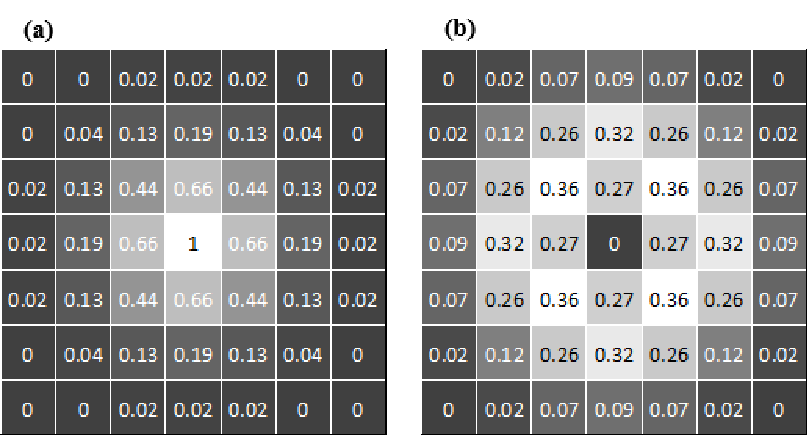
\includegraphics[width=0.6\linewidth]{fig8.pdf}
\caption{The filters which appear in Eq. \ref{H_V_image}. Here, the truncated Gaussian kernel was used, with $\sigma=1.1$ and size $7\times7$.  \textbf{(a)} The filter $K$  \textbf{(b)} The filter $L$}
\label{filters}
\end{figure}





















\section{Conclusion}
\label{conclusion}
The Parzen probability density function is extracted from a set of data points, and is often used in data analysis. We have shown that it can be decomposed into a product of a weight function and a shape distribution $\Psi\left(\mathbf{x}\right)=W\left(\mathbf{x}\right)S\left(\mathbf{x}\right)$. Whereas many clustering methods are based on probability maxima, as derived through Mean Shift, which coincides with our MPC, we understand that this is far from being the only method of choice based on the Parzen approach. For small values of $\sigma$, $S$ is close to $1$ and therefore MPC should give similar results to MWC. But for larger values of $\sigma$, there exists a difference between the two, and MSC carries interesting additional information. This is indeed borne out by the crab data analysis in Fig. \ref{crabs}. Moreover, this analysis is an example where MSC leads to better results than the other two schemes. One satisfactory advantage of this analysis is that it provides an explanation as to why QC \cite{horn2001}, which coincides with MSC for Gaussian kernels, is a successful algorithm \cite{scott2017data,cui2016analog,liu2016analyzing}.

The understanding which we offer for the success of shape-based clustering (MSC or QC) is that Shape is free of the Weight bias, hence it is sensitive to small changes in the data, and may discover novelties in the data. This is exemplified in Fig. \ref{1d_example}. Note that searching for novelties is a problematic task. For example, a recently proposed method \cite{rodriguez2014clustering} starts with the assumption that ``cluster centers are characterized by a higher density than their neighbors and by a relatively large distance from points with higher densities''. Obviously the toy example demonstrated in Fig. \ref{1d_example} has only a ratio $2$ between the relative distances, yet Shape turned out to be sensitive enough to indicate the existence of the small source!

The dynamical search for clusters is carried out by letting replica-points follow gradient ascent, ending up in cluster centers with which the corresponding data-points are associated. Replica dynamics allow for both unraveling the loci of extrema and associating data points with clusters. We point out that replica dynamics in all three fields can be carried out in a hierarchical fashion, which turns out to result both in lower computational complexity and better intuitive comprehension of the emerging clusters.

A recent review of clustering methods for data analyses \cite{xu2015comprehensive} notes the existence of $45$ commonly used ``modern clustering algorithms'' which it classifies into $10$ classes. There are a few kernel-based clustering algorithms (including SVC), but QC and DQC are classified as ``algorithms based on quantum mechanics''. We believe that one important insight of our current paper is to demystify the connection of QC to quantum mechanics. The relations established here follow naturally from the use of Gaussian kernels. This kernel leads to a Schrődinger equation involving $V$ and $\Psi$ but it does not require any prior assumption involving quantum mechanics.

The three different clustering schemes which we study within our Weight-Shape decomposition scheme, may lead to different results. They can be confronted with expert classifications, using Jaccard scores, thus establishing their qualities. They can also be compared to each other, as well as to themselves (for different scale values), using the same Jaccard procedure.
The relative usefulness of the three families of algorithms depends on the distribution of the data, on dimensionality and on preprocessing. In general we may state that maximal-entropy, which is the principle leading to MWC, reflects the semi-local size properties of the probability distribution, whereas MSC (QC) is sensitive to local shape properties, unbiased by weight. Thus, if one is interested in gross global features, one may be advised to search first the weight component, whereas if one wishes to detect anomalies one should start with the shape distribution.

Applying the Weight-Shape decomposition to image analysis, we realize that, even for small $\sigma$ values of order of $1$ pixel, the shape distribution carries interesting information: it serves as an edge detector. Hence it can be employed for contour drawings of a 2d image. Although neural networks incorporate edge-detection as an inherent feature of their elements, the shape distribution is of interest because it brings in a new tool which is of different nature: a Shape-Filter which is constructed through the division of two convolutional kernels. This single filter has the properties leading to the contour construction which we have exemplifies in line caricatures. The same methodology may facilitate surface searches in 3d images being studied in technical and scientific data. Moreover, this filter may also serve as a novel component to be incorporated in general deep convolutional networks.

The code required to reproduce experiments described in this paper can be found at \url{https://github.com/sliorde/weight-shape-decomposition}.

























\section*{Acknowledgement}
\label{acknowledgments}
We thank S. Zucker for his suggestion of, and help with, the asteroid data analysis.
This research was partially funded by the Blavatnik Cyber Center of Tel Aviv University.

\section*{References}
\bibliographystyle{elsarticle-num} 
\bibliography{references}


\appendix
\section{Crab Data Set}
\label{crab_apndx}
To illustrate field structures at different scales we display in Fig. \ref{crabs_0.3} and Fig. \ref{crabs_0.7} topographic maps of the three functions, together with the original data-points (where different colors indicate different classes in the data). The former figure has $\sigma=0.3$, which gives four clusters in MWC, befitting the maxima of the weight, and the latter figure has $\sigma=0.7$, which gives four clusters in MSC. The complex structure of $W$ provides a natural explanation why the optimal result of $4$ clusters survives for only a short range of $\sigma$.

Finally we display the results of  blurring versions of the three algorithms on the problem at hand. Figs. \ref{crabs_jaccard_blurring} display Jaccard scores and numbers of clusters for the different algorithms, and behave quite similarly to the corresponding MSC, MWC and MPC results in Fig. \ref{crabs}. Fig. \ref{crabs_W_final} displays the blurred field $W$ after convergence of BMWC for $\sigma=0.235$.

\begin{figure}[h]
\centering
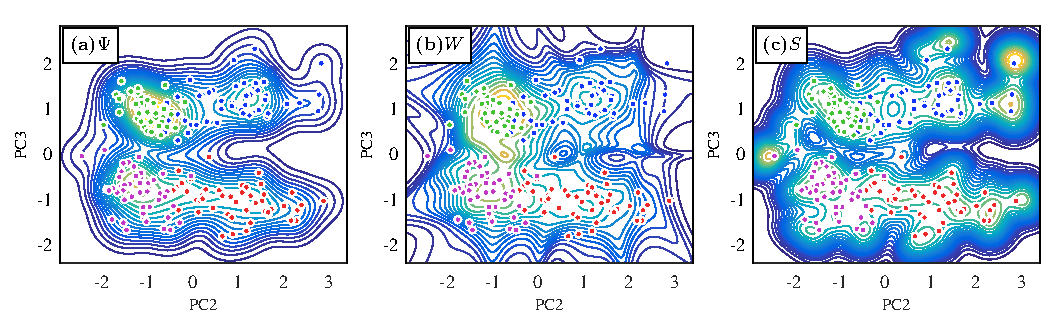
\includegraphics[width=1\linewidth]{fig9.pdf}
\caption{Topographic maps of the three methods for $\sigma= 0.3$}
\label{crabs_0.3}
\end{figure}

\begin{figure}[h]
\centering
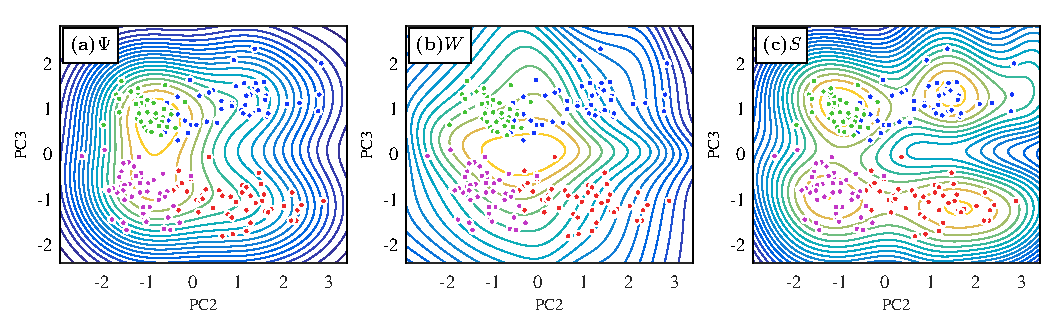
\includegraphics[width=1\linewidth]{fig10.pdf}
\caption{Topographic maps of the three methods for $\sigma= 0.7$}
\label{crabs_0.7}
\end{figure}

\begin{figure}[t]
\centering
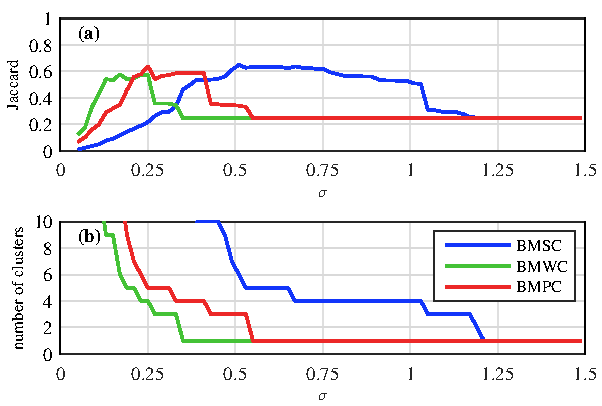
\includegraphics[width=0.6\linewidth]{fig11.pdf}
\caption{Three blurring methods applied to crab data}
\label{crabs_jaccard_blurring}
\end{figure}

\begin{figure}[t]
\centering
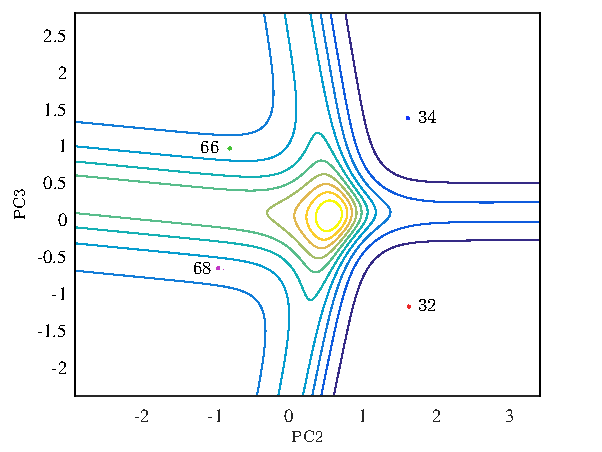
\includegraphics[width=0.6\linewidth]{fig12.pdf}
\caption{Entropy topographic map of the final state of BMWC for $\sigma = 0.235$. The four cluster centers are shown together with the numbers of their assigned data points.}
\label{crabs_W_final}
\end{figure}





In this analysis we have compared the three different clustering schemes with each other, and found that the MSC (or QC) ones do best when judged by the Jaccard score or the $\sigma$ range for which the results are stable. Although there exists here a ground-truth, given by the labels of the data, it should be clear that we have confined ourselves, on purpose, to the $\text{PC2}-\text{PC3}$ representation of the data, which constraints the ability of any of the models, to lead to perfect clustering.

It has become conventional to test clustering methods on artificially designed problems, which are quite difficult for $k$-means to decipher. For examples we refer to \cite{Carreira2015clustering} where a lengthy study of different mean-shift methods is presented, confronting them with such data and with other algorithms. Mean Shift (MS) has the advantage of focusing on densities of the data distribution. Obviously QC also focuses on data distributions. The difference between the two approaches is that QC is free of the bias carried by the Weight, as demonstrated in Fig. \ref{1d_example}. Obviously this plays in favor of QC vs MS (or MSC vs MPC) in the crab analysis. The results of the weight-based approach, MWC, are quite similar to those of MPC, and show best performances for low $\sigma$, where Shape values are small.

The advantage of QC \cite{horn2001} over the kernel-based SVC \cite{ben2001} has already been pointed out in \cite{horn2001}: whereas the kernel-based SVC could not establish reasonable clustering unless it allowed for a very large percentage of outliers, QC has solved it easily. QC has been employed in many applications. A recent review \cite{scott2017data} studies both the crab and other data sets, and demonstrates its advantages.



















\end{document}
\endinput
